
\documentclass{article}
\usepackage{pagecolor}
\definecolor{ultramarine}{RGB}{254, 250, 214} 

\usepackage[showframe]{geometry}
%\usepackage{layout}
\setlength{\headsep}{5pt}
\usepackage{graphicx}
\usepackage{subfig}

\begin{document}
\pagecolor{ultramarine}
\title{Experimental Design}
\author{}
\date{}
\maketitle
\section{Key questions}
For a common arrival and service probability, which system configuration has a lower average waiting time per customer? By subjecting the alternative systems to identical experimental conditions, we hope to make it easy to distinguish which systems are best even though the respective estimators might have sampling error.

\section{Sensitivity Analysis}
The simulation problem is of terminating type, and the initialization conditions (ie., initial queue length) thus have a non-trivial effect on the average waiting time outputted by the model. As such, by varying simulation conditions, we hope to analyze how the resultant average queueing times are affected in the current system configuration.

\section{Simulation Run Structure}
The problem is a comparison of average waiting per customer between two queueing configurations. As such, we take the sample means of the desired simulation output from each system configuration, and identify a confidence interval that establish the difference between the sample means of each configuration. The smaller the sample mean, the better. As such, if the interval lies to the left of the center of the standardized distribution then the first system is better, and if the the interval lies to the right then the alternative system is better. If the interval contains zero, then the performance of both systems are statistically, about the same. The structure is best demonstrated in the figures \ref{IDEF01}, \ref{IDEF02} and \ref{IDEF03} below.
\begin{figure}[h]
  \centering
  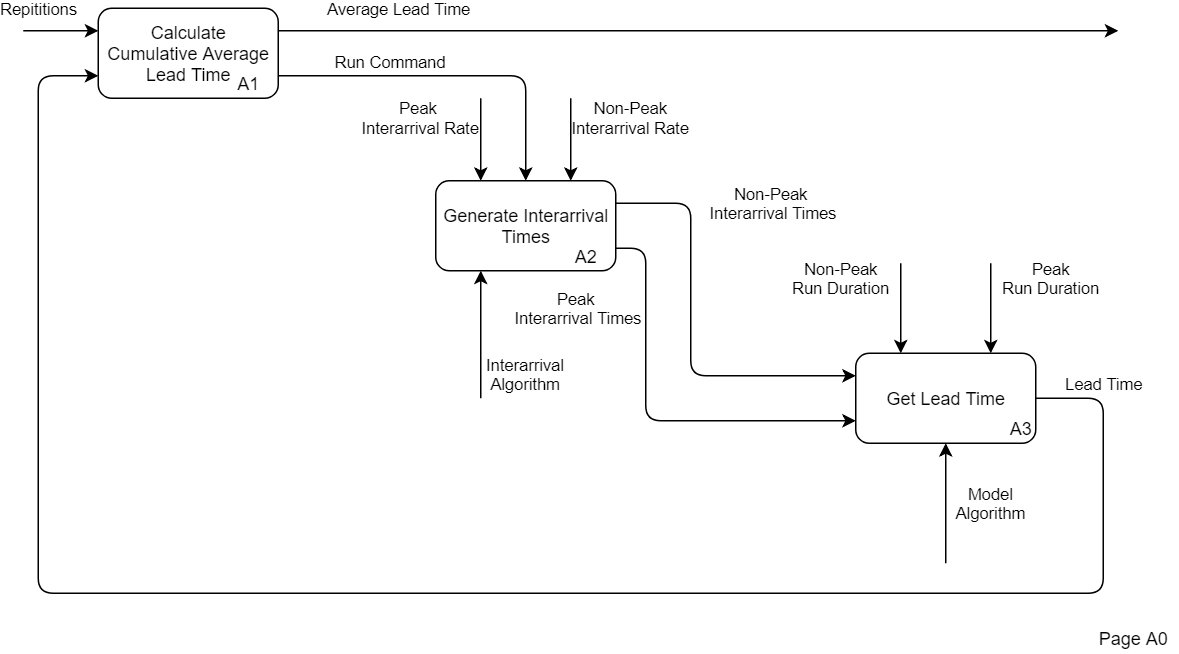
\includegraphics[scale=0.2]
  {A0.png}
  \caption{IDEF0 A0 Page}
  \label{IDEF01}
\end{figure}

\begin{figure}[h]
  \centering
  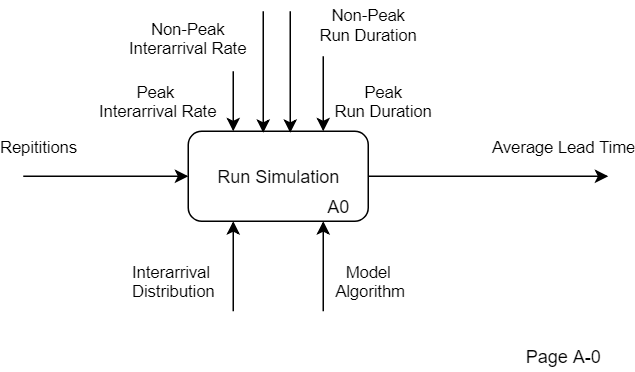
\includegraphics[scale=0.4]
  {A-0.png}
  
  \caption{IDEF0 A-0 Page}
  \label{IDEF02}
\end{figure}

\begin{figure}[h]
  \centering
  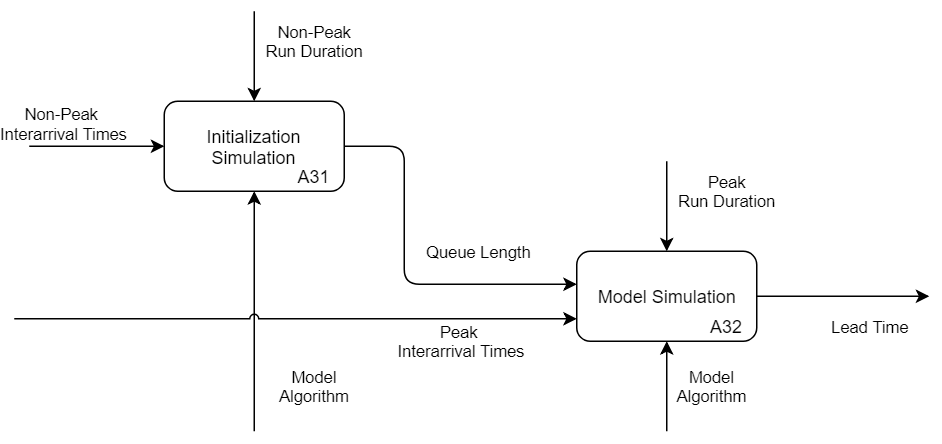
\includegraphics[scale=0.4]
  {A3.png}
  
  \caption{IDEF0 A3 Page}
  \label{IDEF03}
\end{figure}

\section{Simulation Run Duration}
The problem is time constrained as the scope of the project is limited to analyzing queuing behavior comparisons during peak periods. As such, the termination sequence for each run in both simulation models (Initial and alternative queuing system) is conditional on the number of timesteps. (ie., if the each simulation run ends after the time steps are at equal to or greater than the number of time steps that represent a 45 minute time period). The replication sequence of each run terminates after 10,000 iterations

\end{document}